\documentclass[a4paper,12pt]{report}
\usepackage[spanish,mexico]{babel}
\usepackage[utf8]{inputenc}
\usepackage[T1]{fontenc}
\usepackage{amsmath}
\usepackage{amssymb}
\usepackage{wasysym}
\usepackage[dvipsnames,pdftex]{color}
\usepackage[x11names]{xcolor}
\usepackage{tikz, tkz-euclide}
\usepackage[american]{circuitikz}
\usepackage{siunitx}
\usetikzlibrary{arrows}
\usepackage[colorinlistoftodos]{todonotes}
%\usepackage[left=2cm,right=1.5cm,top=1cm,bottom=1cm]{geometry}
%\usepackage{helvet}
%\renewcommand{\familydefault}{\sfdefault}
\setlength{\oddsidemargin}{0in}
\usepackage{geometry}
\geometry{a4paper, total = {180mm,270mm},
			left = 25mm, top = 20mm,
            right=15mm,bottom=20mm,%
            footskip=10mm}
\usepackage{float} 
% \setlength{\topmargin}{0in}
% \setlength{\voffset}{-0.5in}
% \setlength{\hoffset}{0.3in}
% \setlength{\textheight}{700pt}
% \setlength{\textwidth}{440pt}
% \setlength{\topskip}{0in}
% \setlength{\parskip}{2ex}
 \renewcommand{\baselinestretch}{1.5}
\usepackage{diagbox}
\usepackage{array}
\usepackage{listings}
\usepackage{caption}
%%% comandos definidos por el usuario
\begin{document}
\setcounter{page}{1}
\pagenumbering{roman}
\thispagestyle{empty}
\begin{center}
{\huge UNIVERSIDAD NACIONAL DE INGENIERÍA}\\[0.9cm]
{\Large FACULTAD DE INGENIERÍA MECÁNICA}\\[0.6in]
\end{center}
\begin{figure}[h]
\begin{center}

\includegraphics[scale=0.33]{logoUNI.png}
\vspace{0cm}
\end{center}
\end{figure}
\vspace{0.5cm}
\begin{center}
INFORME DE LABORATORIO\\
LABORATORIO DE CIRCUITOS ELÉCTRICOS\\[5mm]
{\large USO DEL GENERADOR DE ONDAS Y DEL OSCILOSCOPIO: VALORES CARACTERÍSTICOS DE ONDAS PERIÓDICAS}\\[10mm]
\vfill
LIMA - PERÚ \hfill OCTUBRE 2019
\end{center}
\newpage
\thispagestyle{empty}
\begin{center}
{\Large USO DEL GENERADOR DE ONDAS Y DEL OSCILOSCOPIO: VALORES CARACTERÍSTICOS DE ONDAS PERIÓDICAS}\\[0.7cm]
\small ENTREGADO:\\[0.05cm]
\small 09 OCTUBRE 2019\\[1.2cm]
\end{center}
\begin{flushleft}
{\large ALUMNOS:}\\[2cm]
\end{flushleft}
\begin{center}
\begin{tabular}{c@{\hspace{0.5in}}c}
\rule[1pt]{2.6in}{1pt}&\rule[1pt]{2.6in}{1pt}\\
Garay Altamirano Franklyn, 20130509E & Huaroto Villavicencio Josue, 20174070\\[1.5cm]
\rule[1pt]{2.6in}{1pt}&\rule[1pt]{2.6in}{1pt}\\
Landeo Sosa Bruno, 20172024J & Quesquen Vitor Angel, 20170270C \\[1.5cm]
%Sotelo Cavero Sergio, 20172125K & Nombre 5, 2017 \\[1.5cm]
\end{tabular}
\end{center}
%\begin{center}
%\begin{tabular}{c@{\hspace{0.6in}}c}
%\rule[1pt]{3.14in}{1pt}\\
%Huaroto Villavicencio Josué, 20174070I \\[2cm]
%\rule[1pt]{3.14in}{1pt}\\
%Landeo Sosa Bruno, 20174070I \\[2cm]
%\rule[1pt]{3.14in}{1pt}\\
%Quesquén Vitor Angel, 20172125K \\[2cm]
%\rule[1pt]{3.14in}{1pt}\\
%Sotelo Cavero Sergio, 20172125K \\[2cm]
%\end{tabular}
%\end{center}
\begin{center}
\begin{tabular}{c}
\rule[1pt]{3.14in}{1pt}\\
Sotelo Cavero Sergio, 20172125K\\[2.5cm]
\end{tabular}
\end{center}

%\rule[1pt]{3.14in}{1pt}\\
%Maguiña Amaya Wladimir, 20172019F \\[3cm]
%\rule[1pt]{3.14in}{1pt}\\
%Luis Sosa Jose, 19774147I \\[3cm]
%\rule[1pt]{3.14in}{1pt}\\
%Sotelo Cavero Sergio, 20172125K
%\end{tabular}
%\end{center}
%\\[0.7cm]
{\large PROFESOR:} \\[2cm]
\begin{center}
\begin{tabular}{c}
\rule[3pt]{4.8in}{1pt}\\[1pt]
ING. SINCHI YUPANQUI, FRANCISCO 
\end{tabular}
\end{center}
\vfill
%\newpage
%\begin{center}
%{\Large \bf{RESUMEN}}
%\end{center}
\newpage
\tableofcontents
%\listoffigures
%\addcontentsline{toc}{chapter}{Índice de figuras}
\newpage
\pagenumbering{arabic} %%% esto es para regresar el modo de numeración a numeración arábiga
\setcounter{page}{1}  %%% empezamos en página 1
%\part{Introducción}
\chapter{Objetivos}
\begin{enumerate}
\item Interactuar con los diodos y apreciar su característica restrictiva aplicada a la modificación de una onda.
\item Aprender a utilizar el osciloscopio digital.
\item Comparar los valores medios y eficaces visualizados por el multímetro y osciloscopio con los calculados teóricamente.
\end{enumerate}
\chapter{Marco teórico}
\section{Osciloscopio}
Un osciloscopio es un instrumento de visualización electrónico para la representación gráfica de señales eléctricas que pueden variar en el tiempo. Es muy usado en electrónica de señal, frecuentemente junto a un analizador de espectro. Presenta los valores de las señales eléctricas en forma de coordenadas en una pantalla, en la que normalmente el eje $X$ (horizontal) representa tiempos y el eje $Y$ (vertical) representa tensiones. La imagen así obtenida se denomina oscilograma. Suelen incluir otra entrada, llamada ``eje THRASHER'' o ``Cilindro de Wehnelt'' que controla la luminosidad del haz, permitiendo resaltar o apagar algunos segmentos de la traza.\\
Los osciloscopios, clasificados según su funcionamiento interno, pueden ser tanto analógicos como digitales, siendo el resultado mostrado idéntico en cualquiera de los dos casos.
\subsection{Osciloscopio digital}
En la actualidad los osciloscopios analógicos están siendo desplazados en gran medida por los osciloscopios digitales, entre otras razones por la facilidad de poder transferir las medidas a una computadora personal o pantalla LCD. En el osciloscopio digital la señal es previamente digitalizada por un conversor analógico digital. Al depender la fiabilidad de la visualización de la calidad de este componente, esta debe ser cuidada al máximo.\\
Las características y procedimientos señalados para los osciloscopios analógicos son aplicables a los digitales. Sin embargo, en estos se tienen posibilidades adicionales, tales como el disparo anticipado (pre-triggering) para la visualización de eventos de corta duración, o la memorización del oscilograma transfiriendo los datos a un PC. Esto permite comparar medidas realizadas en el mismo punto de un circuito o elemento. Existen asimismo equipos que combinan etapas analógicas y digitales.\\
La principal característica de un osciloscopio digital es la velocidad de muestreo, la misma determinara el ancho de banda máximo que puede medir el instrumento basándose en el Teorema de Nyquist. Viene expresada en MS/s (millones de samples /muestras/ por segundo).\\
La mayoría de los osciloscopios digitales en la actualidad están basados en control por FPGA (del inglés Field Programmable Gate Array), el cual es el elemento controlador del conversor analógico a digital de alta velocidad del aparato y demás circuitería interna, como memoria, buffers, entre otros.\\
Estos osciloscopios añaden prestaciones y facilidades al usuario imposibles de obtener con circuitería analógica, como los siguientes:
\begin{itemize}
\item Medida automática de valores de pico, máximos y mínimos de señal. Verdadero valor eficaz.
\item Medida de flancos de la señal y otros intervalos.
\item Captura de transitorios.
\item Cálculos avanzados, como la FFT para calcular el espectro de la señal. También sirve para medir señales de tensión.
\item Dentro del osciloscopio digital existen dos tipos que se diferencian claramente:
\end{itemize}
\begin{figure}[H]
\centering
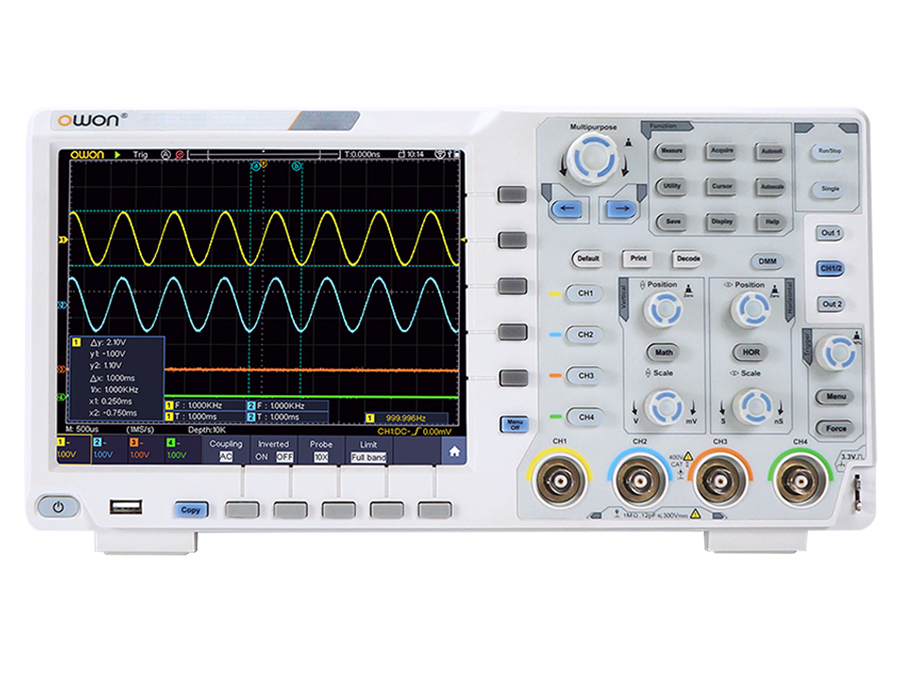
\includegraphics[scale=0.35]{osciloscopio.jpg}
\end{figure}
\section{Función peripodica}
En matemática, una función es periódica si verifica la condición $f(x+T)=f(x)$; el número $T$ se llama periodo de la función. Generalmente, se llama período fundamental al menor número real positivo $T$ que satisface la condición. Las funciones trigonométricas son ejemplos sencillos de una función periódica, que en combinaciones adecuadas se emplean en el análisis armónico. De la misma manera, pero en un contexto físico, las ondas periódicas son aquellas ondas que muestran periodicidad respecto del tiempo, es decir, describen ciclos repetitivos. En una onda periódica se cumple:
$$
x_{a}(t) = x_{a}(t+T_{p}) = x_{a}(t+nT_{p})
$$
donde el periodo propio fundamental $T_{p} = 1/F$, $F$ es la frecuencia de la componente fundamental de la onda periódica y $n$ un número entero. Toda onda periódica es, por definición, una onda determinista, por cuanto puede ser descrita matemáticamente (mediante un modelo matemático).
\begin{figure}[H]
\centering
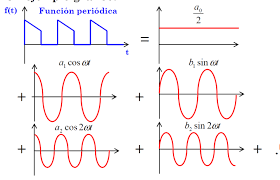
\includegraphics[scale=1.1]{periodica.png}
\end{figure}
\section{Rectificador}
Un rectificador es el dispositivo electrónico que permite convertir la corriente alterna en corriente continua. Esto se realiza utilizando diodos rectificadores, ya sean semiconductores de estado sólido, válvulas al vacío o válvulas gaseosas como las de vapor de mercurio (actualmente en desuso). Dependiendo de las características de la alimentación en corriente alterna que emplean, se les clasifica en monofásicos, cuando están alimentados por una fase de la red eléctrica, o trifásicos cuando se alimentan por tres fases.
Atendiendo al tipo de rectificación, pueden ser de media onda, cuando solo se utiliza uno de los semiciclos de la corriente, o de onda completa, donde ambos semiciclos son aprovechados. El tipo más básico de rectificador es el rectificador monofásico de media onda, constituido por un único diodo entre la fuente de alimentación alterna y la carga.
\begin{figure}[H]
\centering
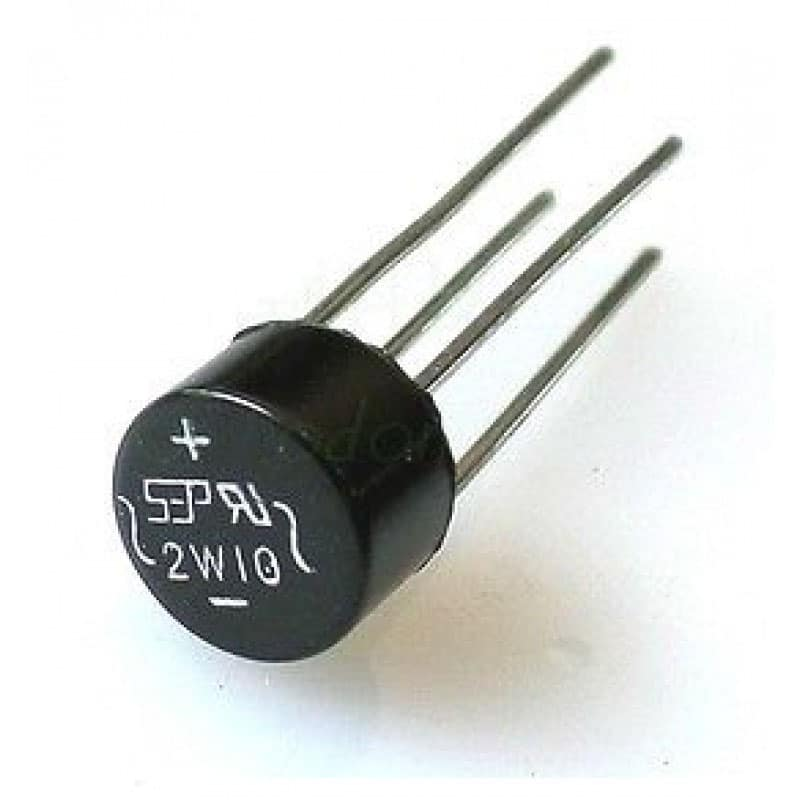
\includegraphics[scale=0.2]{rectificador.jpg}
\end{figure}
\chapter{Cuestionario}
\begin{enumerate}
\item Explicar el principio de funcionamiento del osciloscopio y el generador de ondas. Asimismo enumerar sus diversos usos.\\
Los osciloscopios comprueban y muestran las señales de tensión como formas de onda y como representaciones visuales de la variación de tensión en función del tiempo. Las señales se representan en un gráfico, que muestra cómo cambia la señal. El eje vertical (Y) representa la medición de la tensión, y el eje horizontal (X) representa el tiempo.
El muestreo es el proceso de convertir una parte de una señal de entrada en un número de valores eléctricos discretos con el propósito de almacenarla, procesarla y visualizarla. La magnitud de cada punto de muestra es igual a la amplitud de la señal de entrada en el momento en que la señal es muestreada.
La forma de onda de entrada aparece como una serie de puntos en la pantalla. Si los puntos se encuentran espaciados ampliamente y son difíciles de interpretar como una forma de onda, se pueden conectar usando un proceso llamado interpolación, que conecta los puntos con líneas, o vectores.
Los controles de disparo le permiten estabilizar y mostrar una forma de onda repetitiva.
El disparo por flanco es la forma más común de disparo. En este modo, el nivel de disparo y los controles de pendiente proporcionan la definición básica del punto de disparo. El control de pendiente determina si el punto de disparo se encuentra en el flanco ascendente o descendente de una señal, y el control de nivel determina en qué lugar del flanco se produce el punto de disparo.
Cuando se trabaja con señales complejas, como una serie de pulsos, puede ser necesario usar el disparo por ancho de pulso. Con esta técnica, el ajuste de nivel de disparo y el próximo flanco descendente de la señal deben ocurrir dentro de un lapso de tiempo especificado. Una vez alcanzadas estas dos condiciones, el osciloscopio disparará.
Otra técnica es la de disparo único, en la que el osciloscopio solo mostrará un trazo cuando la señal de entrada cumpla con las condiciones establecidas de disparo. Una vez cumplidas las condiciones de disparo, el osciloscopio adquiere y actualiza la pantalla, y luego congela la pantalla para mantener el trazo.
\subsection*{Uso del osciloscopio}
\begin{enumerate}
\item Determinar directamente el periodo y el voltaje de una señal.
\item Determinar indirectamente la frecuencia de una señal.
\item Determinar que parte de la señal es DC y cual AC.
\item Localizar averías en un circuito.
\item Medir la fase entre dos señales.
\item Determinar que parte de la señal es ruido y como varia este en el tiempo.
\end{enumerate}
\item Explicar el principio de funcionamiento del diodo y del puente de diodos y su aplicación en electricidad. \\
Los primeros diodos que aparecieron eran válvulas o tubos vacíos llamados válvulas termoiónicas y que se encontraban construidos por medio de dos electrodos rodeados de vació en un tubo de cristal, muy similares a las lámparas incandescentes.\\
El que es polarizado directamente permite el flujo a través de él de los electrones, o lo que es lo mismo permite el paso de la corriente eléctrica, en polarización inversa no permite el paso de los electrones por él.
Para tensiones con polarización directa del diodo, según aumentamos la tensión en los bornes del diodo (patillas o extremos) va aumentando la corriente que circula por él.\\
Lógicamente el diodo tendrá una tensión máxima de trabajo que no se podrá sobrepasar porque se quemaría, para tensiones con polarización negativa no conduce y, por lo tanto, por mucho que aumentemos la tensión no se producirá corriente alguna a través del diodo.\\
Como vemos los diodos semiconductores tienen la valiosa propiedad de que los electrones solamente fluyen en una dirección a través de ellos y, como resultado, actúan como unos rectificadores.
Son la estructura fundamental de los semiconductores y muchos otros componentes electrónicos se fabrican teniendo como base a los diodos. Los diodos tienen una estructura electrónica llamada Unión PN, es decir son la unión de un material semiconductor llamado N con otro llamado P.\\
\textbf{Puente de diodos}
Es también llamado puente rectificador de diodos, es un dispositivo formado por cuatro diodos ensamblados de forma que una corriente alterna (AC) conectada a dos de los diodos produce una corriente continua (DC) de salida en los dos diodos restantes. Es un componente eléctrico utilizado en muchos aparatos tanto a nivel industrial como a nivel doméstico, por ejemplo, en los cargadores de los teléfonos móviles.\\
 Para entender cómo funciona un puente rectificador de diodos es necesario primero conocer las diferencias básicas entre corriente alterna y corriente continua y como funciona un diodo. La mayoría de la gente está más que habituada a utilizar baterías en electrodomésticos, juguetes, teléfonos, dispositivos multimedia y otros muchos objetos cotidianos. Una batería es un buen ejemplo de fuente de alimentación de corriente contínua (CC o DC – Direct Current) pues tienen un polo positivo y un polo negativo que nunca cambian, presenta una polaridad continua. Por el contrario, la corriente alterna (CA o AC – Alternating Current) tiene una polaridad que se invierte aproximadamente entre 50 y 60 veces por segundo.\\
Para hacer que funcionen aparatos CC con un suministro de CA es necesario rectificar la polaridad alternante de la corriente CA y producir una corriente con polaridad estable. Sin esta rectificación, la corriente CA podría provocar daños graves en el aparato. En la mayoría de aparatos la rectificación se consigue con un puente de diodos o con un inversor de voltaje.\\
Los diodos son unos dispositivos que permiten el flujo eléctrico en un sólo sentido y cada puente rectificador lleva al menos cuatro. Para que la rectificación de la corriente alterna se produzca hay que conectar los cuatros diodos en una disposición específica, llamada configuración de rectificación, que efectivamente termina con una mitad del ciclo de la corriente alterna de entrada y deja pasar sólo la otra mitad a través del puente, pero siempre con el polo negativo y el positivo saliendo por los mismos diodos.
\begin{figure}[H]
\centering
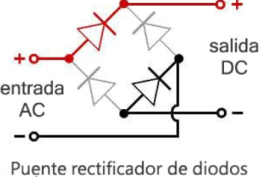
\includegraphics[scale=0.5]{sergod1.png}
\end{figure}
La señal eléctrica generada es forma de pulsos, la llamada media onda de rectificación. Antes de utilizarse es necesario estabilizarla para formar una señal de corriente DC completa, lo que se hace principalmente utilizando condensadores. Finalmente, y si es necesario, la señal puede pasar por un amplificador antes de abandonar el puente.
Los puentes de diodos se utilizan para una amplia gama de aplicaciones. Podemos encontrarlos desde en pequeñas fuentes de alimentación de circuitos electrónicos hasta en grandes aplicaciones industriales que suministran corriente continua a motores y electroimanes. El tamaño de los diodos y los demás componentes del puente cambian según las necesidades de cada aplicación, pero la disposición y construcción permanece muy similar.
Aunque existen otras alternativas para transformar corriente alterna en corriente continua, como los inversores de voltaje, los puentes de diodos siguen siendo la alternativa más barata.
\begin{figure}[H]
\centering
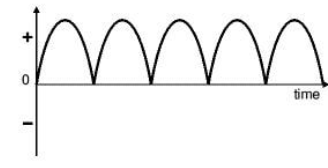
\includegraphics[scale=0.5]{sergod2.png}
\end{figure}
\item Explicar el método empleado para hallar el desfasaje entre voltajes de la fuente y del condensador en un circuito R-C. ¿Qué otros métodos existen?
Para hallar el desfasaje entre voltajes usamos el ociloscopio digital de manera que usamos los 2 canales para identificar las ondas periodicas. En el primer canal conectamos los terminales del condensador y en el segundo conectamos los terminales del voltaje. Acomodamos y superponemos las graficas y obtenemos el valor del desfasaje.\\
\item Elaborar un cuadro de los valores eficaces y medios visualizados en el multímetro, osciloscopio y los calculados teóricamente por fórmulas, indicando \% de error.
\begin{figure}[H]
\centering
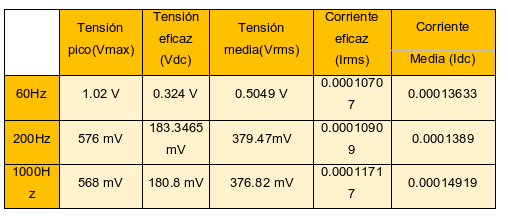
\includegraphics[scale=0.7]{kgda1.png}
\end{figure}
\begin{figure}[H]
\centering
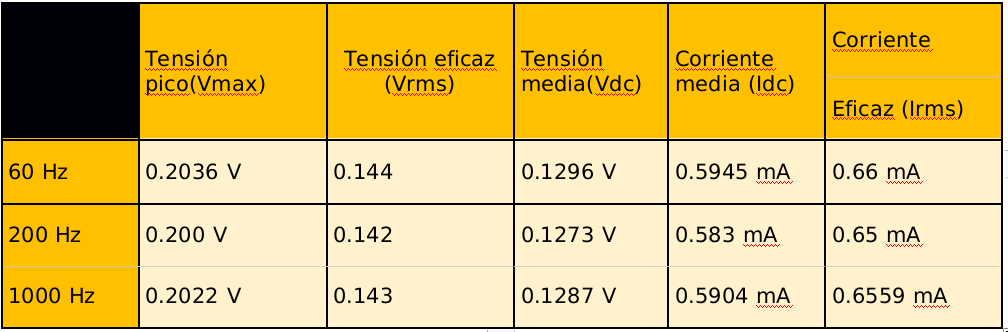
\includegraphics[scale=0.45]{kgda2.png}
\end{figure}

\end{enumerate}
\chapter{Conclusiones y recomendaciones}
\begin{enumerate}
\item Se concluyó que el puente de diodos usado tiene aplicaciones óptimas.
\item En el laboratorio el primer puente de diodos que obtuvimos no estuvo en buenas condiciones, al cambiar de puente se pudo apreciar las gráficas demandadas.
\item El osciloscopio y generador de ondas deben estar en buen estado para que no exista un problema con las frecuencias que se manden uno al otro.
\item El puente de diodos al estar malogrados afecta las frecuencias emitidas en el osciloscopio y no muestra la onda que se necesita por ello debe observar si los puentes de diodos estan en buen estado.
\item Los cables deben engancharse bien entre si sino se perdera las graficas sinusoidales en el osciloscopio.
\end{enumerate}
\begin{thebibliography}{99}  %%%este es un contador para el número de bibliografías utilizados.
\addcontentsline{toc}{chapter}{Bibliograf\'{\i}a} %%% Para introducir la bibliografía en el índice.
%\bibitem{Rahman}{Rahman,Aminur y Doe, Hidekazu; ``Ion transfer of tetraalkylammonium cations at an interface between 
%frozen aqueous solution and 1,2-dichloroethane".{\em{Journal of Electroanalytical Chemistry}} {\bfseries 424},159,(1997).}
\bibitem{Gro}{Boylestad, Robert M. ``Introducción al análisis de circuitos''. {\em{Pearson}}}
\bibitem{Gro}{Sadiku, Matthew N. ``Fundamemtos de circuitos eléctricos''. {\em{Mc Graw Hill}}}
%\bibitem{Ding}{Ding, Zhifeng. ``Spectroelectrochemistry and photoelectrochemistry of charge transfer at liquid/liquid
%interfaces". {\em {Tesis, EPFL,}}(1999).}
%\bibitem{AL}{Alonso, Jose M. \em{Técnicas de mecanizado 1}}
%\bibitem{AL}{Alonso, Jose M. ``Técnicas de mecanizado 1". {\em{Paraninfo}} {\bfseries España-Madrid}, 6-20, (2001).}
%\bibitem{Samec2}{Samec Z., Lhotsky A., Jänchenová H., y Marecek, V. ``Interfacial tension and impedance measurements
%of interfaces between two inmiscible electrolyte solutions". {\em{Journal of Electroanalytical Chemistry}} {\bfseries
%43}, 47, (2000).}
%\bibitem{Day}{Day R.A. y Underwood A.L. {\textit{Química Analítica Cuantitativa}},5ºed. Prentice-Hall, México, 1998. 45-48.}
%\bibitem{Keyser}{Farah Abud, Michel. ``Determinación de la vida útil en herramientales de corte endurecido por el proceso de borurización en pasta''. {\em{Instituto tecnológico y de estudios superiores de Monterrey}}}
%\bibitem{Zolotorevski}{Escalona, I. ``Máquinas: herramientas por arranque de viruta.''.{\em{El Cid Editor.}}}
%\bibitem{Lasheras}{Lasheras. ``Tecnología de los Materiales Industriales''.} 
%\bibitem{Dieter}{Dieter. ``Metalurgia mecánica''.}
%\bibitem{Apraiz}{Apraiz, J. ``Tratamiento Térmico de los Aceros''.}
%\bibitem{Smith}{Smith, William F. y Ph.D. Hashemi, Javad ``Ciencia e ingeniería de materiales". {\em{
%Madrid: McGraw-Hill, Interamericana de España.}} 570, (2004).} 
%\bibitem{Callister}{Callister, William D. y Rethwisch, David G. ``Introducción a la ingeniería de los materiales''. %{\em{Barcelona Reverté.}}, 960, (2007).} 
%\bibitem{Askeland}{Askeland, Donald R., Pradeep P. Phulé y Wright, Wendelin J. ``Ciencia e ingeniería de los materiales''.{\em{México, D.F. Internacional Thomson Editores.}} {\textit{$6^{ta}$ edición}}, 1004, (2012).}
%\bibitem{HARDBANDING}{Tabla de conversión de escala de durezas. \begin{verbatim}http://%hardbandingsolutions.com/postle_sp/hardness.php
%\end{verbatim}}
\bibitem{HE}{Apuntes circuitos transitorios. \begin{verbatim} http://users.df.uba.ar/moreno/cursos/lab3/apuntes/transitorios.pdf
\end{verbatim}}
%\bibitem{ASTM}{Normas ASTM.}
%\bibitem{NTP}{Normas NTP.}
\end{thebibliography}
\end{document}